% SC3099 — Chapter 3: System Design — Architecture, UML, and Prototyping
% No \documentclass — included by modules/SC3099/main.tex (book class).
\chapter{System Design: Architecture, UML, and Prototyping}
\label{ch:design}

\begin{quote}
\emph{``Architecture is the decisions you wish you could get right early.''} --- Ralph Johnson. Before a line of production code, design turns requirements into a blueprint that balances change, scale, and clarity.
\end{quote}

\noindent\fbox{\parbox{\dimexpr\linewidth-2\fboxsep-2\fboxrule}{%
\textbf{From zero: we build here, no prior design course needed.} This chapter defines \emph{architecture}, \emph{model}, and \emph{prototype} from first principles---pictures before formalism. We assume only Ch.~2 (requirements): given \emph{what} the system must do, we now decide \emph{how} it is structured, drawn, and validated before coding.}}
\vspace{0.4em}

\section*{Learning Outcomes}
After this chapter you will be able to:
\begin{enumerate}[label=(L\arabic*)]
    \item compare layered, MVC, and microservice architectures and select among them for a capstone-scale system;
    \item read and sketch UML class and sequence diagrams with correct multiplicities and message types;
    \item distinguish low-fidelity from high-fidelity prototypes and plan an iterative Figma-based workflow;
    \item explain coupling versus cohesion and apply the SOLID preview to judge a design;
    \item translate a class diagram into a Python skeleton and trace a use case through layers.
\end{enumerate}

% ============================================================
\section{Architecture Styles: Layered, MVC, and Microservices}
\label{sec:architecture-styles}
Think of a building: foundation, floors, and roof each have a job and only touch neighbours. Software \emph{architecture} is the same---a high-level partition into parts plus the rules for how they may interact. Good architecture makes the inevitable change cheap and localised.

\paragraph{Layered (n-tier).} The classic capstone choice. Requests flow \emph{down} through layers; no layer skips its immediate neighbour. Three layers suffice for most student projects: Presentation (UI), Business Logic, Data Access.

\begin{figure}[h]
\centering
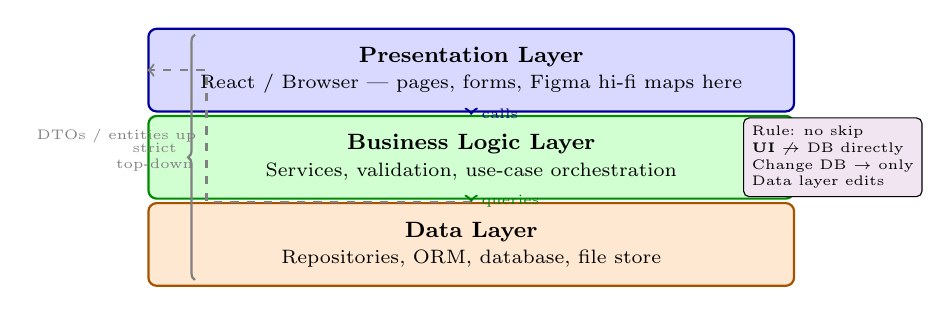
\begin{tikzpicture}[scale=0.82, every node/.style={font=\footnotesize}]
  \tikzstyle{layer}=[draw, thick, rounded corners=3pt, minimum width=8.2cm, minimum height=1.05cm, align=center]
  \node[layer, fill=blue!15, draw=blue!60!black] (pres) at (0,2.4) {\textbf{Presentation Layer} \\ \scriptsize React / Browser --- pages, forms, Figma hi-fi maps here};
  \node[layer, fill=green!18, draw=green!55!black] (biz) at (0,1.05) {\textbf{Business Logic Layer} \\ \scriptsize Services, validation, use-case orchestration};
  \node[layer, fill=orange!18, draw=orange!65!black] (data) at (0,-0.30) {\textbf{Data Layer} \\ \scriptsize Repositories, ORM, database, file store};
  \draw[->, thick, blue!60!black] (pres.south) -- (biz.north) node[midway,right,font=\tiny] {calls};
  \draw[->, thick, green!50!black] (biz.south) -- (data.north) node[midway,right,font=\tiny] {queries};
  \draw[->, thick, dashed, gray] (data.north) -- ++(-4.1,0) |- (pres.west) node[pos=0.25,left,font=\tiny] {DTOs / entities up};
  \node[draw, fill=violet!10, rounded corners=2pt, font=\tiny, align=left, inner sep=3pt] at (5.6,1.05) {Rule: no skip\\ \textbf{UI} $\not\to$ DB directly\\ Change DB $\to$ only\\ Data layer edits};
  \draw[decoration={brace,mirror,raise=3pt},decorate,thick,gray] (-4.15,2.95) -- (-4.15,-0.85) node[midway,left,font=\tiny,align=center] {strict\\ top-down};
\end{tikzpicture}
\caption{Layered architecture --- three coloured tiers with strict top-down dependency. Blue (presentation) depends on green (logic) depends on orange (data); responses flow back as DTOs. Violating the skip rule creates hidden coupling.}
\label{fig:layered-architecture}
\end{figure}

\paragraph{MVC.} Model--View--Controller splits the presentation tier itself: \emph{Model} holds data and rules, \emph{View} renders, \emph{Controller} handles input and updates the Model. The View observes the Model (Observer pattern). Ideal when the same data has multiple views (web + mobile). In Fig.~\ref{fig:layered-architecture}, MVC lives entirely inside the blue layer.

\paragraph{Microservices.} Decompose by business capability into independently deployable services communicating via APIs/events. Gains independent scaling and team ownership; costs are distributed transactions, eventual consistency, and DevOps overhead. For a 3--5 person capstone with one database and tight deadline, a \emph{modular monolith} (well-partitioned layered app) usually beats premature microservices---you can still extract a service later at a module boundary.

\textbf{Choosing.} Ask: team size, scaling needs, and failure isolation. If all data fits one DB and deploy is single-instance, choose layered/MVC. If two subsystems must scale or fail independently (e.g., real-time chat vs.\ grading engine), consider one extracted service, not ten.

\begin{table}[h]
\centering\small
\begin{tabular}{@{}lccc@{}}
\toprule
Concern & Layered & MVC & Microservices \\
\midrule
Team size & 3--5 ideal & 2--5 & 6+ (per service) \\
Deploy units & 1 & 1 & $N$ services \\
Data ownership & Single DB & Single DB & DB per service \\
Consistency & ACID simple & ACID simple & Eventual / Saga \\
When to use & Capstone default & Multiple views & Independent scale \\
\bottomrule
\end{tabular}
\caption{Architecture trade-offs at a glance. Start layered; extract only when a bounded context earns independence.}
\label{tab:arch-tradeoffs}
\end{table}

% ============================================================
\section{UML Essentials: Class and Sequence Diagrams}
\label{sec:uml-essentials}
UML is a sketching language, not bureaucracy. Two diagrams carry 80\% of design value: class diagrams (static structure) and sequence diagrams (dynamic interaction).

\paragraph{Class diagrams} show classes, attributes, operations, and relationships: association (solid line), aggregation (hollow diamond), composition (filled diamond), inheritance (hollow triangle), multiplicity (\texttt{1}, \texttt{0..1}, \texttt{*}, \texttt{1..*}). Fig.~\ref{fig:class-associations} models a capstone ordering domain.

\begin{figure}[h]
\centering
\begin{tikzpicture}[scale=0.75, every node/.style={font=\scriptsize}]
  \tikzstyle{cls}=[draw, thick, rounded corners=2pt, minimum width=2.9cm, align=center]
  \node[cls, fill=blue!15, draw=blue!60!black] (user) at (0,2.6) {\textbf{User}\\ \rule{2.5cm}{0.4pt}\\ \texttt{-userId: String}\\ \texttt{-email: String}\\ \rule{2.5cm}{0.4pt}\\ \texttt{+placeOrder(): Order}};
  \node[cls, fill=green!15, draw=green!55!black] (order) at (5.2,2.6) {\textbf{Order}\\ \rule{2.5cm}{0.4pt}\\ \texttt{-orderId: String}\\ \texttt{-status: Status}\\ \rule{2.5cm}{0.4pt}\\ \texttt{+total(): double}\\ \texttt{+pay(): void}};
  \node[cls, fill=orange!15, draw=orange!65!black] (item) at (5.2,0.15) {\textbf{OrderItem}\\ \rule{2.5cm}{0.4pt}\\ \texttt{-qty: int}\\ \texttt{-price: double}\\ \rule{2.5cm}{0.4pt}};
  \node[cls, fill=violet!12, draw=violet!60!black] (prod) at (0,0.15) {\textbf{Product}\\ \rule{2.5cm}{0.4pt}\\ \texttt{-sku: String}\\ \texttt{-stock: int}\\ \rule{2.5cm}{0.4pt}\\ \texttt{+inStock(): bool}};
  \node[cls, fill=teal!12, draw=teal!60!black] (pay) at (2.6,-1.85) {\textbf{Payment}\\ \rule{2.5cm}{0.4pt}\\ \texttt{-method: String}\\ \texttt{-amount: double}\\ \rule{2.5cm}{0.4pt}\\ \texttt{+process(): bool}};
  % associations
  \draw[thick] (user) -- (order) node[midway,above,font=\tiny] {1 --- *} node[midway,below,font=\tiny,align=center] {places};
  \draw[thick] (order) -- (item) node[midway,right,font=\tiny] {1 --- 1..*} node[midway,left,font=\tiny] {\texttt{<>} composes};
  \node[draw,diamond,fill=black,aspect=1.4,inner sep=2pt] at (5.2,1.38) {};
  \draw[thick] (prod) -- (item) node[midway,above,font=\tiny] {1 --- *} node[midway,below,font=\tiny] {refers to};
  \draw[thick,dashed,->] (order) -- (pay) node[midway,sloped,above,font=\tiny] {uses};
  \draw[thick] (user.east) -- ++(0.3,0) |- (prod.west);
  \node[draw,diamond,fill=white,draw=black,thick,aspect=1.4,inner sep=2pt] at (0,1.38) {};
  \node[font=\tiny,gray,align=center] at (2.6,1.05) {hollow = aggregation\\ filled = composition};
\end{tikzpicture}
\caption{Class diagram with coloured classes and associations. User aggregates Product (wishlist, hollow diamond---independent lifecycle) but Order \emph{composes} OrderItem (filled diamond---items die with order). Multiplicities and a dependency to Payment are explicit.}
\label{fig:class-associations}
\end{figure}

Reading Fig.~\ref{fig:class-associations}: a \texttt{User} places \texttt{*} orders; each \texttt{Order} composes \texttt{1..*} items; each \texttt{OrderItem} refers to one \texttt{Product}. The hollow diamond on User--Product means deleting a User does not delete the Product catalog; the filled diamond on Order--OrderItem means it does. Check every association for multiplicity at \emph{both} ends.

\paragraph{Sequence diagrams} add time (top to bottom). Lifelines are vertical dashes; horizontal arrows are messages (filled = synchronous/blocking, open = asynchronous, dashed = return). Add \texttt{alt}/\texttt{loop}/\texttt{opt} fragments for branching. A good sequence diagram maps one use case end-to-end: \texttt{User -> Controller -> Service -> Repository -> DB} and back. Keep to 5--7 lifelines; split complex flows rather than nesting fragments three deep.

\begin{lstlisting}[language=Python, caption={Python skeleton generated from the class diagram. Note types, composition, and delegation.}]
from dataclasses import dataclass, field
from typing import List

@dataclass
class Product:
    sku: str
    stock: int
    def in_stock(self) -> bool:
        return self.stock > 0

@dataclass
class OrderItem:
    product: Product
    qty: int
    price: float

@dataclass
class Order:
    order_id: str
    status: str = "PENDING"
    items: List[OrderItem] = field(default_factory=list)
    def total(self) -> float:
        return sum(i.qty * i.price for i in self.items)
    def pay(self, payment: "Payment") -> bool:
        if payment.process():
            self.status = "PAID"
            return True
        return False

@dataclass
class Payment:
    method: str
    amount: float
    def process(self) -> bool:
        # delegate to gateway; return True on success
        return True
\end{lstlisting}

Translate associations faithfully: composition becomes owned list field (\texttt{Order.items}); aggregation becomes a reference that outlives the owner; inheritance becomes subclassing; multiplicities become \texttt{List} vs.\ single reference vs.\ \texttt{Optional}.

% ============================================================
\section{Prototyping: Low-Fi to Hi-Fi and Iterative Design}
\label{sec:prototyping}
A prototype is a cheap, partial system built to answer a question before the answer is expensive. Fidelity is the question of \emph{how close to real}.

\paragraph{Low-fi} (paper, whiteboard, wireframes): boxes and labels, no colour, no real data. Cost is minutes; purpose is to test \emph{flow} and \emph{information architecture}. Best for the first stakeholder review---stakeholders critique structure, not colours.

\paragraph{Hi-fi} (Figma, clickable): pixel-accurate, real copy, interactive transitions, design-system components. Cost is hours; purpose is to test \emph{usability} and to hand off specs to developers (spacing, colours, states). Link frames into a clickable flow and run a 5-user hallway test.

\begin{table}[h]
\centering\small
\begin{tabular}{@{}lcc@{}}
\toprule
 & Low-fi & Hi-fi (Figma) \\
\midrule
Looks like & Boxes \& labels & Pixel-accurate UI \\
Time to build & Minutes & Hours \\
What it tests & Flow, IA, scope & Usability, visual, handoff \\
When & Sprint~0 / kickoff & Before coding feature \\
Audience & Stakeholders, team & Users, developers \\
\bottomrule
\end{tabular}
\caption{Low-fi versus hi-fi: choose fidelity to match the question you need answered cheaply.}
\label{tab:prototype-fidelity}
\end{table}

\begin{figure}[h]
\centering
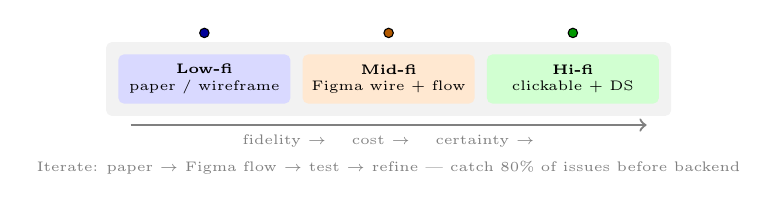
\begin{tikzpicture}[scale=0.78, every node/.style={font=\scriptsize}]
  % fidelity spectrum bar
  \fill[gray!10, rounded corners=2pt] (0,0) rectangle (9.2,1.2);
  \fill[blue!15, rounded corners=2pt] (0.2,0.2) rectangle (3.0,1.0);
  \fill[orange!18, rounded corners=2pt] (3.2,0.2) rectangle (6.0,1.0);
  \fill[green!18, rounded corners=2pt] (6.2,0.2) rectangle (9.0,1.0);
  \node[align=center, font=\tiny] at (1.6,0.6) {\textbf{Low-fi}\\ paper / wireframe};
  \node[align=center, font=\tiny] at (4.6,0.6) {\textbf{Mid-fi}\\ Figma wire + flow};
  \node[align=center, font=\tiny] at (7.6,0.6) {\textbf{Hi-fi}\\ clickable + DS};
  \draw[->, thick, gray] (0.4,-0.15) -- (8.8,-0.15) node[midway,below,font=\tiny] {fidelity $\to$ \quad cost $\to$ \quad certainty $\to$};
  \node[draw, circle, fill=blue!60!black, inner sep=1.2pt] at (1.6,1.35) {};
  \node[draw, circle, fill=orange!70!black, inner sep=1.2pt] at (4.6,1.35) {};
  \node[draw, circle, fill=green!60!black, inner sep=1.2pt] at (7.6,1.35) {};
  \node[font=\tiny, gray, align=center] at (4.6,-0.85) {Iterate: paper $\to$ Figma flow $\to$ test $\to$ refine --- catch 80\% of issues before backend};
\end{tikzpicture}
\caption{Prototyping fidelity spectrum. Move right only when the cheaper level has answered its question; each step trades more build time for higher certainty.}
\label{fig:fidelity-spectrum}
\end{figure}

\paragraph{Iterative loop.} Prototype $\to$ review $\to$ measure $\to$ refine. In Figma, keep a single design system (colours, typography, components) so hi-fi iterations are cheap. Two to three cycles typically catch 80\% of usability issues before any backend exists. For capstone, gate your sprints: no coding of a feature until its hi-fi flow is signed off in Figma, and no hi-fi polish until the low-fi flow is validated.

% ============================================================
\section{Design Principles: Coupling, Cohesion, and SOLID Preview}
\label{sec:design-principles}
Two words predict maintenance cost:

\begin{itemize}
    \item \textbf{Coupling} --- how much a module depends on others. Lower is better. Data coupling (passing values) beats stamp, control, and content coupling.
    \item \textbf{Cohesion} --- how focused a module's responsibilities are. Higher is better. Functional cohesion (one purpose) beats sequential, communicational, and coincidental.
\end{itemize}

\paragraph{SOLID preview} (detailed in SC2006 Ch.~4): \textbf{S}ingle Responsibility (one reason to change), \textbf{O}pen/Closed (extend without editing), \textbf{L}iskov Substitution (subtypes must be substitutable), \textbf{I}nterface Segregation (small focused interfaces), \textbf{D}ependency Inversion (depend on abstractions). In Fig.~\ref{fig:layered-architecture}, DIP appears as the Presentation depending on a \texttt{OrderService} \emph{interface}, not a concrete \texttt{MySQLOrderStore}---this is what lets you test the controller with a fake store and swap databases without touching business logic.

\begin{itemize}
    \item \textbf{SRP:} \texttt{ReportManager} that prints, queries, and emails should be three classes.
    \item \textbf{OCP:} Add new payment types by adding a class, not editing \texttt{if-else} chains.
    \item \textbf{LSP/ISP/DIP:} Accept \texttt{PaymentGateway} interface; any gateway (Stripe, PayNow) plugs in and mocks for tests.
\end{itemize}

\begin{remark}
Heuristic: if changing one requirement forces edits in three layers, your boundaries are wrong. Repackage by \emph{feature} (vertical slice: Order feature owns its UI, service, and repo) rather than by technical layer when the team is small. Prefer composition over inheritance and keep hierarchies shallow (depth $\le 3$).
\end{remark}

% ============================================================
\section{Exercises}
\label{sec:ch03-exercises}
\begin{enumerate}[label=E3.\arabic*, leftmargin=*, itemsep=0.6em]
    \item \textbf{Layered vs.\ microservices.} Your capstone is a 4-person team building an event-booking app with one PostgreSQL database, due in 12~weeks. Argue for a modular monolith. Identify one future condition that would justify extracting a single microservice and name its bounded context and API.
    \item \textbf{Class diagram repair.} A diagram shows \texttt{Order} --\texttt{*}-- \texttt{Product} with no association class and multiplicity \texttt{1..*} at both ends. Explain what information is lost (quantity, price snapshot) and redraw with \texttt{OrderItem} and correct multiplicities and diamond fills.
    \item {\sloppy \textbf{Sequence to code.} Draw a sequence diagram for ``user pays for order'' across \texttt{Browser -> OrderController -> OrderService -> PaymentGateway -> Database} with an \texttt{alt} fragment for payment success/failure. Then list the method signatures that each arrow implies.\par}
    \item \textbf{Coupling and cohesion analysis.} A class \texttt{ReportManager} generates PDFs, queries the DB, and sends emails. Identify its cohesion level and coupling type, apply SRP to split it into three classes, and show how DIP lets you unit-test the new \texttt{ReportService} without a real database.
    \item \textbf{Prototype plan.} For a ``student team formation'' feature, outline a two-cycle prototype plan: (a) low-fi wireframes and the three questions they must answer, (b) hi-fi Figma flow and a 5-user test task with success criteria, (c) what you would \emph{not} prototype in either cycle and why.
\end{enumerate}
